
\chapter{Methodology}
\label{ch:methodology}

This chapter presents the methodology used to create the dataset, train the neural network, and perform the adversarial attack. 

\section{Baseline conception}

We need to conceptualize a baseline since we are starting the project without previous work. The baseline is the starting point of the project. It is the simplest system that we can create to solve the problem. We can then use the baseline to compare our results and improve the system.

We conceptualized the baseline of the system as follows: we place the microphones on the side of the road, and the sound source is the vehicle. The microphones record the sound emitted by the vehicles driving on the road. The sound source localization system then detects the vehicle's position. The setup of the baseline is shown in Figure \ref{fig:baseline_setup}.

\begin{figure}[H]
    \centering
    \subfloat[\centering Side view]{{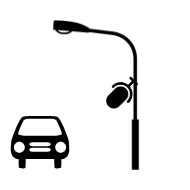
\includegraphics[width=5cm]{../Images/setup_side_view.drawio.png} }}%
    \qquad
    \subfloat[\centering Top down view]{{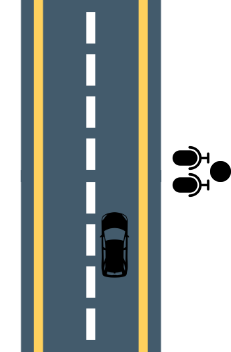
\includegraphics[width=5cm]{../Images/setup_top_down_view.drawio.png} }}%
    \caption{Setup of the baseline}%
    \label{fig:baseline_setup}%
\end{figure}

Using microphones and an embedded system to detect vehicle positions is an efficient and effective way of providing a real-time sound source localization system. This idea can be further developed to incorporate other sound sources for movement tracking in a generalized environment, such as emergency vehicle detection. The baseline is a valuable starting point to develop and test a system that can accurately identify and track sound sources.

Overall, the baseline provides a context to develop further a concept of an accurate sound source localization system for outdoor space. The setup can be easily replicated in many other environments, such as other city streets, traffic intersections, etc. This setup is a valuable starting point to develop and test a system that can accurately identify and track sound sources.

\subsection{Dataset conception}

The dataset is the most crucial part of the baseline. We can determine the dataset's characteristics based on the analysis of the section \ref{sec:datasetsSSL}. The dataset needs to contain the sound recorded by the microphone and the position of the sound source. To simplify the problem, we will use four classes as the main classification challenge in the project. The classes are the following:

\begin{itemize}
    \item  \textit{left\_to\_right}: The vehicle goes from the left to the right of the microphone.
    \item  \textit{right\_to\_left}:  The vehicle goes from the right to the left of the microphone.
    \item  \textit{no\_cars}:  No vehicles pass by the microphone.
    \item  \textit{multiple\_cars}:  Multiple vehicles pass by the microphone.
\end{itemize}

By adding a camera to the system, we can use the image captured by the camera to determine the ground truth of the sound source's position. The camera's position is the same as the microphone's position, and the camera is facing the road. These classes allow the creation of a dataset without precisely recording the vehicle's position. The \textit{no\_cars} and \textit{multiple\_cars} are here to ensure we will have a complete dataset, as with these four classes, we can cover every possible scenario recorded by the microphones and don't need to cherry-pick only the recordings that match our classification system. 

We also used only two classes at the beginning of the project to ensure the concept's functionality when installing the system. These classes are the following:

\begin{itemize}
    \item  \textit{left\_to\_right}:  The vehicle goes from the left to the right of the microphone.
    \item  \textit{right\_to\_left}:  The vehicle goes from the right to the left of the microphone.
\end{itemize}

% TODO add appendix
The results and comparison of this task are available in the appendix ??????????.

\subsection{Real data retrieval system conception}

To record real data that suits our baseline 

\subsection{Data recording and storage}

\section{Convolutional Neural Network for Sound Source Localization}

\section{Adversarial Attack conception}

\section{Sound Propagation Simulation}





\subsection{Audio reconstruction from spectrograms}

Since the adversarial example is a spectrogram, it needs to be converted back into audio to be recorded again through the microphone. The conversion is done using the Griffin-Lim algorithm\cite{griffin1984signal}. The Griffin-Lim algorithm is an algorithm that reconstructs an audio signal from a spectrogram. It is an iterative algorithm that uses the spectrogram to estimate the phase of the audio signal. The algorithm starts with a random phase and iteratively updates the phase until the spectrogram converges to the original spectrogram. The algorithm is defined as follows: